The details of the numerical setup are presented in Section \ref{mms}.

We wish to use $Q_1 \times Q_1$ element, which, unless stabilised,
violates  the LBB stability condition and therefore is unusable. 
Stabilisation can be of two types: least-squares \cite{dohu03,temr92,kibr12,gubl07},
or by means of an additional term in the weak form as first introduced in \cite{dobo04,bodg06}, 
which is appealing since there is no explicit satabilisation parameter.
It is further analysed in \cite{nosi01,lihc09,hufb86,shry78,grcc95}.
Note that an equal-order velocity-pressure formulation that does not exhibit spurious
pressure modes (without stabilisaion) has been presented in \cite{risc86}.

This element corresponds to bilinear velocities, bilinear pressure 
(equal order interpolation for both velocity and pressure) which is 
very convenient in terms of data structures since all dofs are colocated.

In geodynamics, it is used in the Rhea code \cite{stgb10,busa13} and in Gale \cite{arbi13}.
It is also used in \cite{lezh11} in its stabilised form, in conjunction with AMR. 
This element is quickly discussed at page 217 of Volker John's book \cite{john16}.

The stabilisation term $\C$ enters the Stokes matrix in the (2,2) position:
\[
\left(
\begin{array}{cc}
\K & \G \\ \G^T & -\C 
\end{array}
\right)
\cdot
\left(
\begin{array}{c}
{\cal V} \\ {\cal P}
\end{array}
\right)
=
\left(
\begin{array}{c}
 f \\ h
\end{array}
\right)
\]
The purpose of the $\C$ term is to stabilise the linear system. It is given by:
\[
\C(p,q) = \sum_e \int_{\Omega_e} \frac{1}{\eta} (p-\Pi p)(q-\Pi q) d\Omega
\]
where $\Pi$ is the $L^2$-projection onto the space of element-wise constant functions:
\[
\Pi p = \frac{1}{|\Omega_e|}\int_{\Omega_e} p d\Omega
\]
Because of the stabilisation matrix $\C$, the numerical solution satisfies the incompressibility
condition only approximately. Local mesh refinement helps to control these unwanted effects
\cite{bugs09,busa13}.
Since $\K$ and $\C$ are symmetric matrices, the Stokes system is then an indefinite symmetric system.
The Schur complement matrix $\SSS$ is then given by 
\[
\SSS = \G^T \cdot \K^{-1}\cdot \G + \C
\]
One can further expand the above expression for the $\C$ term:
\begin{eqnarray}
\C(p,q) 
&=& \sum_e \int_{\Omega_e} \frac{1}{\eta} (p-\Pi p)(q-\Pi q) d\Omega \nonumber\\
&=& \sum_e \int_{\Omega_e} \frac{1}{\eta} [ pq - (\Pi p)q -(\Pi q)p + (\Pi p)(\Pi q)] d\Omega \nonumber\\
&=& \sum_e \frac{1}{\eta_e} \left[  
\int_{\Omega_e} pq   d\Omega -\int_{\Omega_e} (\Pi p)q d\Omega 
-\int_{\Omega_e} (\Pi q)p  d\Omega +  \int_{\Omega_e}   (\Pi p)(\Pi q) d\Omega \right] \nonumber\\
&=& \sum_e \frac{1}{\eta_e} \left[  
\int_{\Omega_e} pq   d\Omega - (\Pi p) \int_{\Omega_e} q d\Omega 
- (\Pi q) \int_{\Omega_e} p  d\Omega +  (\Pi p)(\Pi q)  \int_{\Omega_e}  d\Omega \right] \nonumber\\
&=& \sum_e \frac{1}{\eta_e} \left[  
\int_{\Omega_e} pq   d\Omega 
- (\Pi p) |\Omega_e| (\Pi q) 
- (\Pi q) |\Omega_e| (\Pi p) 
+ (\Pi p)(\Pi q) |\Omega_e| \right] \nonumber\\
&=& \sum_e \frac{1}{\eta_e} \left[  
\int_{\Omega_e} pq   d\Omega 
- |\Omega_e| (\Pi p) (\Pi q) 
\right]
\end{eqnarray}
where we have used the fact that on each element $\Pi p^h$ is constant. 
The left term will obviously yield a $Q_1$ mass matrix (scaled by the elemental viscosities).
Note that this approach is not used in practice as we'll see hereafter. 

The pressure inside an element is given by 
\[
p^h(\vec x) = \sum_k N_k^p(\vec x) p_k
\]
so that 
\begin{eqnarray}
\Pi p^h 
&=& \frac{1}{|\Omega_e|} \int_{\Omega_e} \sum_k N_k^p p_k d\Omega 
= \sum_k \left(\underbrace{\frac{1}{|\Omega_e|} \int_{\Omega_e} N_k^p  d\Omega}_{\tilde{N}_k^p} \right) p_k
\end{eqnarray}
and then
\[
p^h -\Pi p^h 
= \sum_k N_k^p(\vec x) p_k - \sum_k \tilde{N}_k^p p_k  
= \sum_k (N_k^p(\vec x) - \tilde{N}_k^p) p_k  
\]
The algorithm is straighforward and as follows:
In the loop over elements, a) Compute the average of each shape function $N_k^p(\vec x)$ over the element;
b) Substract this average to the shape function; c) Build mass matrix with modified/offset shape functions
(taking in account the viscosity).
 
In the case of rectangular elements of size $(h_x,h_y)$, $\tilde{N}_k^p$ simplifies even more:
\begin{eqnarray}
\tilde{N}_k^p 
&=& \frac{1}{|\Omega_e|} \int_{\Omega_e} N_k^p(\vec x)   d\Omega  
= \frac{1}{h_xh_y} \frac{h_xh_y}{4} \int_{-1}^{+1} \int_{-1}^{+1} N_k^p(r,s)   drds 
= \frac{1}{4} \int_{-1}^{+1} \int_{-1}^{+1} N_k^p(r,s)   drds 
\end{eqnarray}
It is easy to show that the average of the $Q_1$ shape functions of over the reference 
element is 1, so that $ \tilde{N}_k^p=1/4$. 
This explains why in the code we have:
\begin{lstlisting}
Navrg = np.zeros(m,dtype=np.float64)
Navrg[0]=0.25
Navrg[1]=0.25
Navrg[2]=0.25
Navrg[3]=0.25
\end{lstlisting}
This also means that $\Pi p^h = (p_1+p_2+p_3+p_4)/4$, i.e. the projected pressure
is the mean of the vertex values. It follows, as shown on p.244 of \cite{elsw} that 
the elemental $\C$ matrix is (omitting the viscosity term)
\[
\C_{el} = \mathbb{M}_{el} - \vec q^T \vec q |\Omega_e| \qquad\qquad 
\vec q=\left(\frac{1}{4},\frac{1}{4},\frac{1}{4},\frac{1}{4} \right)
\]
The nullspace of $\C$ consists of constant vectors, i.e. $\vec 1 \in \text{null}(\C)$ which means
that the assembled stabilisation operator is consistent.

The elemental $\C_{el}$ matrix is then computed like a mass matrix, although with modified 
shape function vectors. Inside the loop over quadrature points, we do:
\begin{lstlisting}
Nvect[0,0:m]=N[0:m]-Navrg[0:m]
C_el+=Nvect.T.dot(Nvect)*jcob*weightq/viscosity(xq,yq,case)
\end{lstlisting}
It is then assembled inside the big FEM matrix 
\begin{lstlisting}
for k1 in range(0,m):
    for k2 in range(0,m):
        C_mat[icon[k1,iel],icon[k2,iel]]+=C_el[k1,k2] 
\end{lstlisting}

\noindent
\underline{Non-zero pattern of the $\G$ matrix}: Let us take a simple example: a 3x2 element grid.

\begin{center}
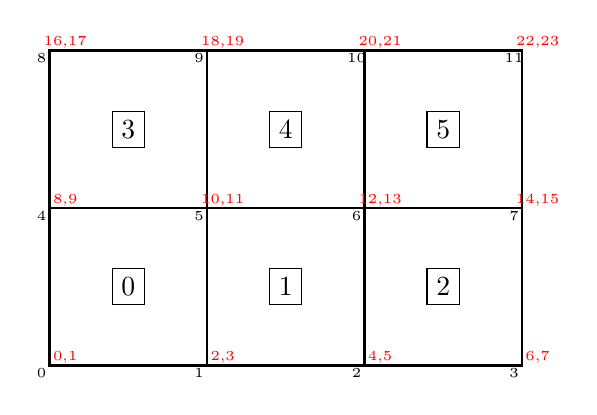
\begin{tikzpicture}
%\draw[step=0.5cm,gray,very thin] (0,0) grid (8,6); %background grid
\draw[thick] (1,1) -- (3,1) -- (3,3) -- (1,3) -- cycle;  
\draw[thick] (3,1) -- (5,1) -- (5,3) -- (3,3) -- cycle; 
\draw[thick] (5,1) -- (7,1) -- (7,3) -- (5,3) -- cycle; 
\draw[thick] (1,3) -- (3,3) -- (3,5) -- (1,5) -- cycle;  
\draw[thick] (3,3) -- (5,3) -- (5,5) -- (3,5) -- cycle; 
\draw[thick] (5,3) -- (7,3) -- (7,5) -- (5,5) -- cycle; 
\node[draw] at (2,2) {0};
\node[draw] at (4,2) {1};
\node[draw] at (6,2) {2};
\node[draw] at (2,4) {3};
\node[draw] at (4,4) {4};
\node[draw] at (6,4) {5};
%pressure dofs
\node at (0.9,0.9) {\tiny 0};
\node at (2.9,0.9) {\tiny 1};
\node at (4.9,0.9) {\tiny 2};
\node at (6.9,0.9) {\tiny 3};
\node at (0.9,2.9) {\tiny 4};
\node at (2.9,2.9) {\tiny 5};
\node at (4.9,2.9) {\tiny 6};
\node at (6.9,2.9) {\tiny 7};
\node at (0.9,4.9) {\tiny 8};
\node at (2.9,4.9) {\tiny 9};
\node at (4.9,4.9) {\tiny 10};
\node at (6.9,4.9) {\tiny 11};
%velocity dofs
\node[red] at (1.2,1.1) {\tiny 0,1};
\node[red] at (3.2,1.1) {\tiny 2,3};
\node[red] at (5.2,1.1) {\tiny 4,5};
\node[red] at (7.2,1.1) {\tiny 6,7};
\node[red] at (1.2,3.1) {\tiny 8,9};
\node[red] at (3.2,3.1) {\tiny 10,11};
\node[red] at (5.2,3.1) {\tiny 12,13};
\node[red] at (7.2,3.1) {\tiny 14,15};
\node[red] at (1.2,5.1) {\tiny 16,17};
\node[red] at (3.2,5.1) {\tiny 18,19};
\node[red] at (5.2,5.1) {\tiny 20,21};
\node[red] at (7.2,5.1) {\tiny 22,23};

\end{tikzpicture}
\end{center}

The $\K$ matrix is of size $NfemV \times NfemV$ with $NfemV=ndofV \times nnp = 2\times 12=24$.
The $\G$ matrix is of size $NfemV \times NfemP$ with $NfemP=ndofP \times nnp = 1\times 12=12$.
The $\C$ matrix is of size $NfemP \times NfemP$. 

A corner pdof sees 4 vdofs, a side pdof sees 12 vdofs and an inside pdof sees 18 vdofs, so that 
the total number of nonzeros in $\G$ can be computed as follows:
\[
NZ_\G = \underbrace{4}_{corners} + 
\underbrace{2(nnx-2)*12}_{2 hor. sides} 
+ 
\underbrace{2(nny-2)*12}_{2 vert. sides} 
+ 
\underbrace{(nnx-2)(nny-2)*18}_{inside nodes}
\]
Concretely, 
\begin{itemize}
\item pdof $\#0$ sees vdofs 0,1,2,3,8,9,10,11
\item pdof $\#1$ sees vdofs 0,1,2,3,4,5,8,9,10,11,12,13
\item pdof $\#5$ sees vdofs 0,1,2,3,4,5,8,9,10,11,12,13,16,17,18,19,20,21
\end{itemize}
so that the $\G^T$ matrix non-zero structure then is as follows:
\begin{center}
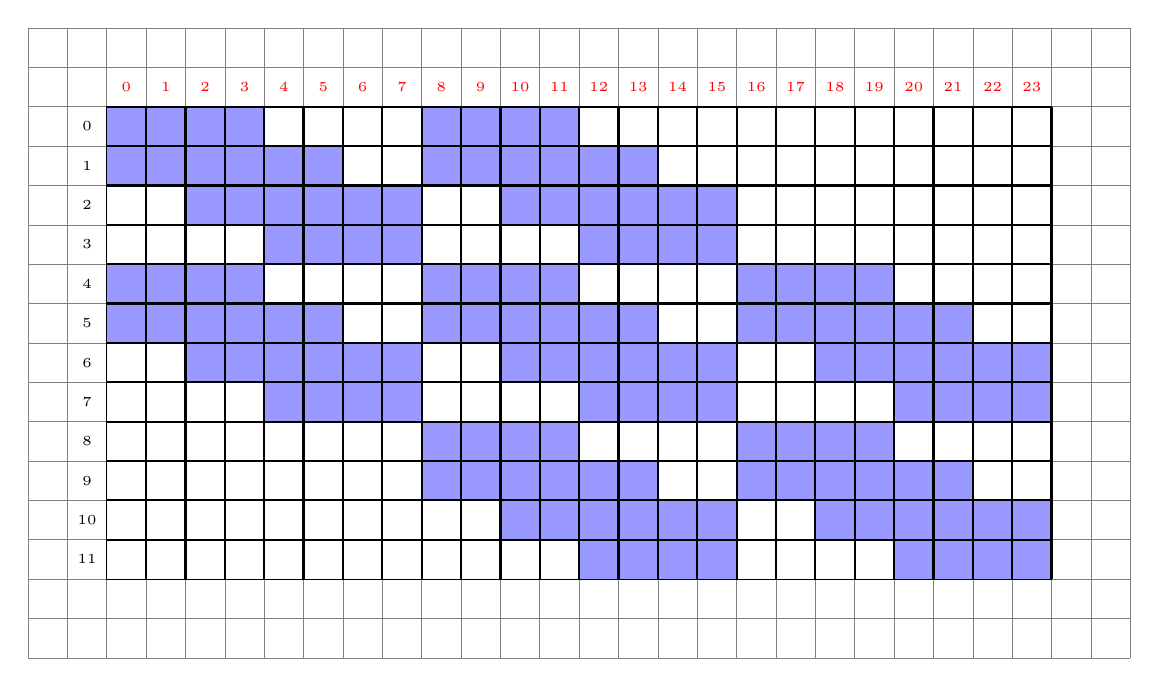
\begin{tikzpicture}
\draw[step=0.5cm,gray,very thin] (0,0) grid (14,8); %background grid
\draw (1,1) -- (13,1) -- (13,7) -- (1,7) -- cycle;    %matrix
%first top line
\fill[blue!40!white] (1.0,6.5) rectangle (1.5,7);
\fill[blue!40!white] (1.5,6.5) rectangle (2.0,7);
\fill[blue!40!white] (2.0,6.5) rectangle (2.5,7);
\fill[blue!40!white] (2.5,6.5) rectangle (3.0,7);
\fill[blue!40!white] (5.0,6.5) rectangle (5.5,7);
\fill[blue!40!white] (5.5,6.5) rectangle (6.0,7);
\fill[blue!40!white] (6.0,6.5) rectangle (6.5,7);
\fill[blue!40!white] (6.5,6.5) rectangle (7.0,7);
%second line
\fill[blue!40!white] (1.0,6.) rectangle (1.5,6.5);
\fill[blue!40!white] (1.5,6.) rectangle (2.0,6.5);
\fill[blue!40!white] (2.0,6.) rectangle (2.5,6.5);
\fill[blue!40!white] (2.5,6.) rectangle (3.0,6.5);
\fill[blue!40!white] (3.0,6.) rectangle (3.5,6.5);
\fill[blue!40!white] (3.5,6.) rectangle (4.0,6.5);
\fill[blue!40!white] (5.0,6.) rectangle (5.5,6.5);
\fill[blue!40!white] (5.5,6.) rectangle (6.0,6.5);
\fill[blue!40!white] (6.0,6.) rectangle (6.5,6.5);
\fill[blue!40!white] (6.5,6.) rectangle (7.0,6.5);
\fill[blue!40!white] (7.0,6.) rectangle (7.5,6.5);
\fill[blue!40!white] (7.5,6.) rectangle (8.0,6.5);
%third line
\fill[blue!40!white] (2.0,5.5) rectangle (2.5,6.0);
\fill[blue!40!white] (2.5,5.5) rectangle (3.0,6.0);
\fill[blue!40!white] (3.0,5.5) rectangle (3.5,6.0);
\fill[blue!40!white] (3.5,5.5) rectangle (4.0,6.0);
\fill[blue!40!white] (4.0,5.5) rectangle (4.5,6.0);
\fill[blue!40!white] (4.5,5.5) rectangle (5.0,6.0);
\fill[blue!40!white] (6.0,5.5) rectangle (6.5,6.0);
\fill[blue!40!white] (6.5,5.5) rectangle (7.0,6.0);
\fill[blue!40!white] (7.0,5.5) rectangle (7.5,6.0);
\fill[blue!40!white] (7.5,5.5) rectangle (8.0,6.0);
\fill[blue!40!white] (8.0,5.5) rectangle (8.5,6.0);
\fill[blue!40!white] (8.5,5.5) rectangle (9.0,6.0);
%fourth line
\fill[blue!40!white] (3.0,5.) rectangle (3.5,5.5);
\fill[blue!40!white] (3.5,5.) rectangle (4.0,5.5);
\fill[blue!40!white] (4.0,5.) rectangle (4.5,5.5);
\fill[blue!40!white] (4.5,5.) rectangle (5.0,5.5);
\fill[blue!40!white] (7.0,5.) rectangle (7.5,5.5);
\fill[blue!40!white] (7.5,5.) rectangle (8.0,5.5);
\fill[blue!40!white] (8.0,5.) rectangle (8.5,5.5);
\fill[blue!40!white] (8.5,5.) rectangle (9.0,5.5);
%fifth line
\fill[blue!40!white] (1.0,4.5) rectangle (1.5,5);
\fill[blue!40!white] (1.5,4.5) rectangle (2.0,5);
\fill[blue!40!white] (2.0,4.5) rectangle (2.5,5);
\fill[blue!40!white] (2.5,4.5) rectangle (3.0,5);
\fill[blue!40!white] (5.0,4.5) rectangle (5.5,5);
\fill[blue!40!white] (5.5,4.5) rectangle (6.0,5);
\fill[blue!40!white] (6.0,4.5) rectangle (6.5,5);
\fill[blue!40!white] (6.5,4.5) rectangle (7.0,5);
\fill[blue!40!white] (9.0,4.5) rectangle (9.5,5);
\fill[blue!40!white] (9.5,4.5) rectangle (10.0,5);
\fill[blue!40!white] (10.0,4.5) rectangle (10.5,5);
\fill[blue!40!white] (10.5,4.5) rectangle (11.0,5);

%sixth line
\fill[blue!40!white] (1.0,4) rectangle (1.5,4.50);
\fill[blue!40!white] (1.5,4) rectangle (2.0,4.50);
\fill[blue!40!white] (2.0,4) rectangle (2.5,4.50);
\fill[blue!40!white] (2.5,4) rectangle (3.0,4.50);
\fill[blue!40!white] (3.0,4) rectangle (3.5,4.50);
\fill[blue!40!white] (3.5,4) rectangle (4.0,4.50);


\fill[blue!40!white] (5.0,4) rectangle (5.5,4.50);
\fill[blue!40!white] (5.5,4) rectangle (6.0,4.50);
\fill[blue!40!white] (6.0,4) rectangle (6.5,4.50);
\fill[blue!40!white] (6.5,4) rectangle (7.0,4.50);
\fill[blue!40!white] (7.0,4) rectangle (7.5,4.50);
\fill[blue!40!white] (7.5,4) rectangle (8.0,4.50);

\fill[blue!40!white] (9.0,4) rectangle (9.5,4.50);
\fill[blue!40!white] (9.5,4) rectangle (10.0,4.50);
\fill[blue!40!white] (10.0,4) rectangle (10.5,4.50);
\fill[blue!40!white] (10.5,4) rectangle (11.0,4.50);
\fill[blue!40!white] (11.0,4) rectangle (11.5,4.50);
\fill[blue!40!white] (11.5,4) rectangle (12.0,4.50);




%seventh line
\fill[blue!40!white] (2.0,3.5) rectangle (2.5,4.0);
\fill[blue!40!white] (2.5,3.5) rectangle (3.0,4.0);
\fill[blue!40!white] (3.0,3.5) rectangle (3.5,4.0);
\fill[blue!40!white] (3.5,3.5) rectangle (4.0,4.0);
\fill[blue!40!white] (4.0,3.5) rectangle (4.5,4.0);
\fill[blue!40!white] (4.5,3.5) rectangle (5.0,4.0);
\fill[blue!40!white] (6.0,3.5) rectangle (6.5,4.0);
\fill[blue!40!white] (6.5,3.5) rectangle (7.0,4.0);
\fill[blue!40!white] (7.0,3.5) rectangle (7.5,4.0);
\fill[blue!40!white] (7.5,3.5) rectangle (8.0,4.0);
\fill[blue!40!white] (8.0,3.5) rectangle (8.5,4.0);
\fill[blue!40!white] (8.5,3.5) rectangle (9.0,4.0);
\fill[blue!40!white] (10.0,3.5) rectangle (10.5,4.0);
\fill[blue!40!white] (10.5,3.5) rectangle (11.0,4.0);
\fill[blue!40!white] (11.0,3.5) rectangle (11.5,4.0);
\fill[blue!40!white] (11.5,3.5) rectangle (12.0,4.0);
\fill[blue!40!white] (12.0,3.5) rectangle (12.5,4.0);
\fill[blue!40!white] (12.5,3.5) rectangle (13.0,4.0);
%eighth line
\fill[blue!40!white] (3.0,3.) rectangle (3.5,3.5);
\fill[blue!40!white] (3.5,3.) rectangle (4.0,3.5);
\fill[blue!40!white] (4.0,3.) rectangle (4.5,3.5);
\fill[blue!40!white] (4.5,3.) rectangle (5.0,3.5);
\fill[blue!40!white] (7.0,3.) rectangle (7.5,3.5);
\fill[blue!40!white] (7.5,3.) rectangle (8.0,3.5);
\fill[blue!40!white] (8.0,3.) rectangle (8.5,3.5);
\fill[blue!40!white] (8.5,3.) rectangle (9.0,3.5);
\fill[blue!40!white] (11.0,3.) rectangle (11.5,3.5);
\fill[blue!40!white] (11.5,3.) rectangle (12.0,3.5);
\fill[blue!40!white] (12.0,3.) rectangle (12.5,3.5);
\fill[blue!40!white] (12.5,3.) rectangle (13.0,3.5);
%9th line
\fill[blue!40!white] (5.0,2.5) rectangle (5.5,3);
\fill[blue!40!white] (5.5,2.5) rectangle (6.0,3);
\fill[blue!40!white] (6.0,2.5) rectangle (6.5,3);
\fill[blue!40!white] (6.5,2.5) rectangle (7.0,3);
\fill[blue!40!white] (9.0,2.5) rectangle (9.5,3);
\fill[blue!40!white] (9.5,2.5) rectangle (10.0,3);
\fill[blue!40!white] (10.0,2.5) rectangle (10.5,3);
\fill[blue!40!white] (10.5,2.5) rectangle (11.0,3);
%10th line
\fill[blue!40!white] (5.0,2) rectangle (5.5,2.5);
\fill[blue!40!white] (5.5,2) rectangle (6.0,2.5);
\fill[blue!40!white] (6.0,2) rectangle (6.5,2.5);
\fill[blue!40!white] (6.5,2) rectangle (7.0,2.5);
\fill[blue!40!white] (7.0,2) rectangle (7.5,2.5);
\fill[blue!40!white] (7.5,2) rectangle (8.0,2.5);
\fill[blue!40!white] (9.0,2) rectangle (9.5,2.5);
\fill[blue!40!white] (9.5,2) rectangle (10.0,2.5);
\fill[blue!40!white] (10.0,2) rectangle (10.5,2.5);
\fill[blue!40!white] (10.5,2) rectangle (11.0,2.5);
\fill[blue!40!white] (11.0,2) rectangle (11.5,2.5);
\fill[blue!40!white] (11.5,2) rectangle (12.0,2.5);
%11th line
\fill[blue!40!white] (6.0,1.5) rectangle (6.5,2);
\fill[blue!40!white] (6.5,1.5) rectangle (8,2);
\fill[blue!40!white] (7.0,1.5) rectangle (7.5,2);
\fill[blue!40!white] (7.5,1.5) rectangle (8.0,2);
\fill[blue!40!white] (8.0,1.5) rectangle (8.5,2);
\fill[blue!40!white] (8.5,1.5) rectangle (9.0,2);
\fill[blue!40!white] (10.0,1.5) rectangle (10.5,2);
\fill[blue!40!white] (10.5,1.5) rectangle (11.0,2);
\fill[blue!40!white] (11.0,1.5) rectangle (11.5,2);
\fill[blue!40!white] (11.5,1.5) rectangle (12.0,2);
\fill[blue!40!white] (12.0,1.5) rectangle (12.5,2);
\fill[blue!40!white] (12.5,1.5) rectangle (13.0,2);
%12th line
\fill[blue!40!white] (7.0,1.0) rectangle (7.5,1.5);
\fill[blue!40!white] (7.5,1.0) rectangle (8.0,1.5);
\fill[blue!40!white] (8.0,1.0) rectangle (8.5,1.5);
\fill[blue!40!white] (8.5,1.0) rectangle (9.0,1.5);
\fill[blue!40!white] (11.0,1.0) rectangle (11.5,1.5);
\fill[blue!40!white] (11.5,1.0) rectangle (12.0,1.5);
\fill[blue!40!white] (12.0,1.0) rectangle (12.5,1.5);
\fill[blue!40!white] (12.5,1.0) rectangle (13.0,1.5);
%vertical
\node at (0.75,6.75) {\tiny 0};
\node at (0.75,6.25) {\tiny 1};
\node at (0.75,5.75) {\tiny 2};
\node at (0.75,5.25) {\tiny 3};
\node at (0.75,4.75) {\tiny 4};
\node at (0.75,4.25) {\tiny 5};
\node at (0.75,3.75) {\tiny 6};
\node at (0.75,3.25) {\tiny 7};
\node at (0.75,2.75) {\tiny 8};
\node at (0.75,2.25) {\tiny 9};
\node at (0.75,1.75) {\tiny 10};
\node at (0.75,1.25) {\tiny 11};
%horizontal
\node[red] at (1.25,7.25) {\tiny 0};
\node[red] at (1.75,7.25) {\tiny 1};
\node[red] at (2.25,7.25) {\tiny 2};
\node[red] at (2.75,7.25) {\tiny 3};
\node[red] at (3.25,7.25) {\tiny 4};
\node[red] at (3.75,7.25) {\tiny 5};
\node[red] at (4.25,7.25) {\tiny 6};
\node[red] at (4.75,7.25) {\tiny 7};
\node[red] at (5.25,7.25) {\tiny 8};
\node[red] at (5.75,7.25) {\tiny 9};
\node[red] at (6.25,7.25) {\tiny 10};
\node[red] at (6.75,7.25) {\tiny 11};
\node[red] at (7.25,7.25) {\tiny 12};
\node[red] at (7.75,7.25) {\tiny 13};
\node[red] at (8.25,7.25) {\tiny 14};
\node[red] at (8.75,7.25) {\tiny 15};
\node[red] at (9.25,7.25) {\tiny 16};
\node[red] at (9.75,7.25) {\tiny 17};
\node[red] at (10.25,7.25) {\tiny 18};
\node[red] at (10.75,7.25) {\tiny 19};
\node[red] at (11.25,7.25) {\tiny 20};
\node[red] at (11.75,7.25) {\tiny 21};
\node[red] at (12.25,7.25) {\tiny 22};
\node[red] at (12.75,7.25) {\tiny 23};
\draw[step=0.5cm,black,thick] (1,1) grid (13,7); %background grid
\end{tikzpicture}
\end{center}

\noindent
\underline{Non-zero pattern of the $\C$ matrix}: Let us take a simple example: a 3x2 element grid.

\todo[inline]{finish structure of C matrix for q1q1}







We impose $\int p dV=0$ which means that the following constraint is added 
to the Stokes matrix:
\[
\left(
\begin{array}{ccc}
\K & \G & 0\\ 
\G^T & \C & \LLL \\
0 & \LLL^T & 0 
\end{array}
\right)
\cdot
\left(
\begin{array}{c}
{\cal V} \\ {\cal P} \\ \lambda
\end{array}
\right)
=
\left(
\begin{array}{c}
 f \\ h \\ 0
\end{array}
\right)
\]











%-----------------------------------------
\subsection*{The Donea \& Huerta benchmark}

As in \cite{dohu03} we solve the benchmark problem presented in section \ref{mms1}.

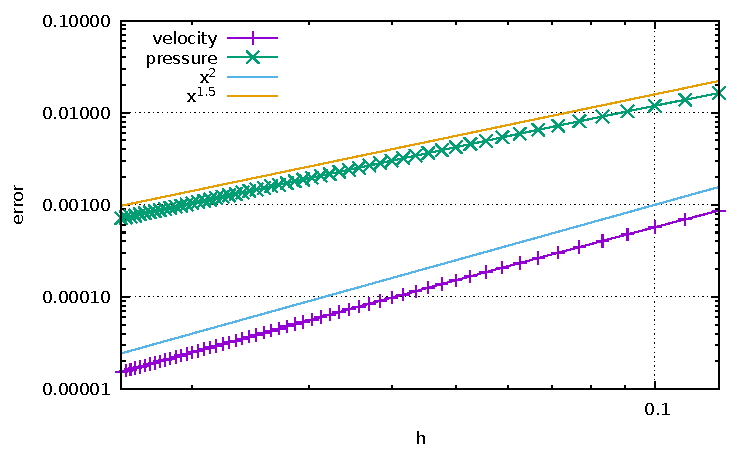
\includegraphics[width=10cm]{python_codes/fieldstone_22/results/case1/errors.pdf}

%-----------------------------------------
\subsection*{The Dohrmann \& Bochev benchmark} 

As in \cite{dobo04} we solve the benchmark problem presented in section \ref{mms2}.

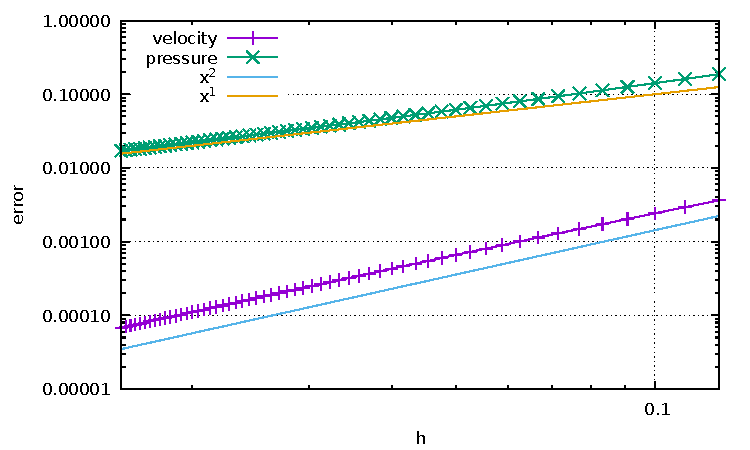
\includegraphics[width=10cm]{python_codes/fieldstone_22/results/case2/errors.pdf}

\todo[inline]{compare my rates with original paper!}

%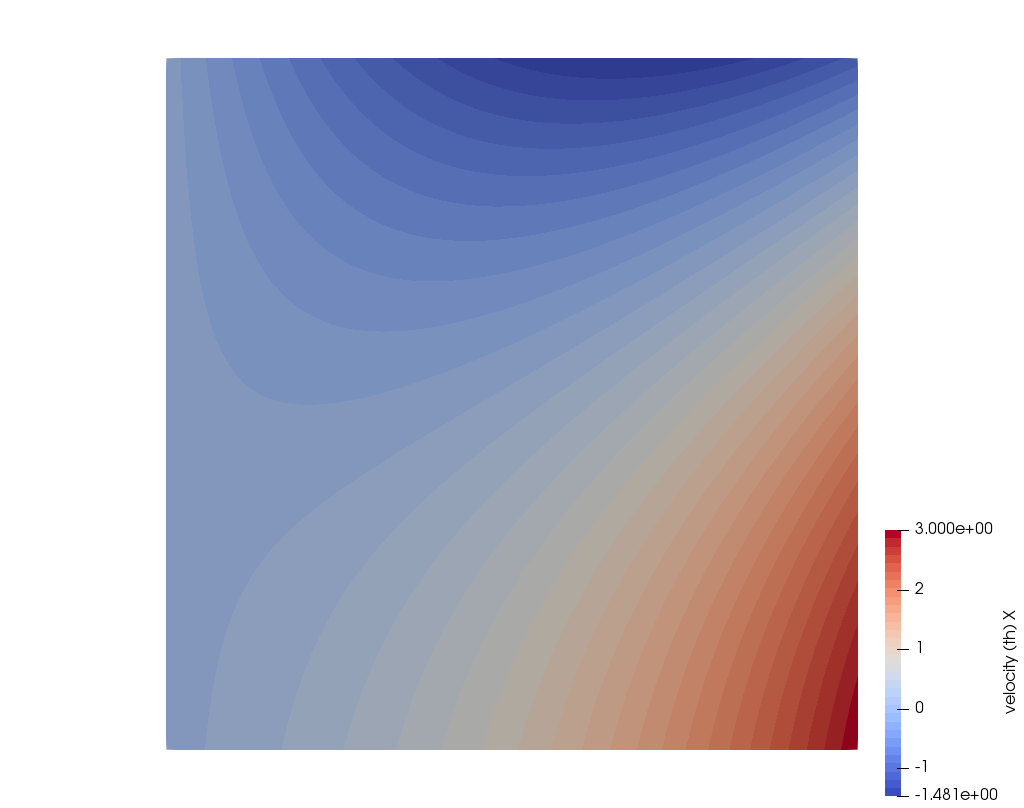
\includegraphics[width=5cm]{python_codes/fieldstone_22/results/uth}
%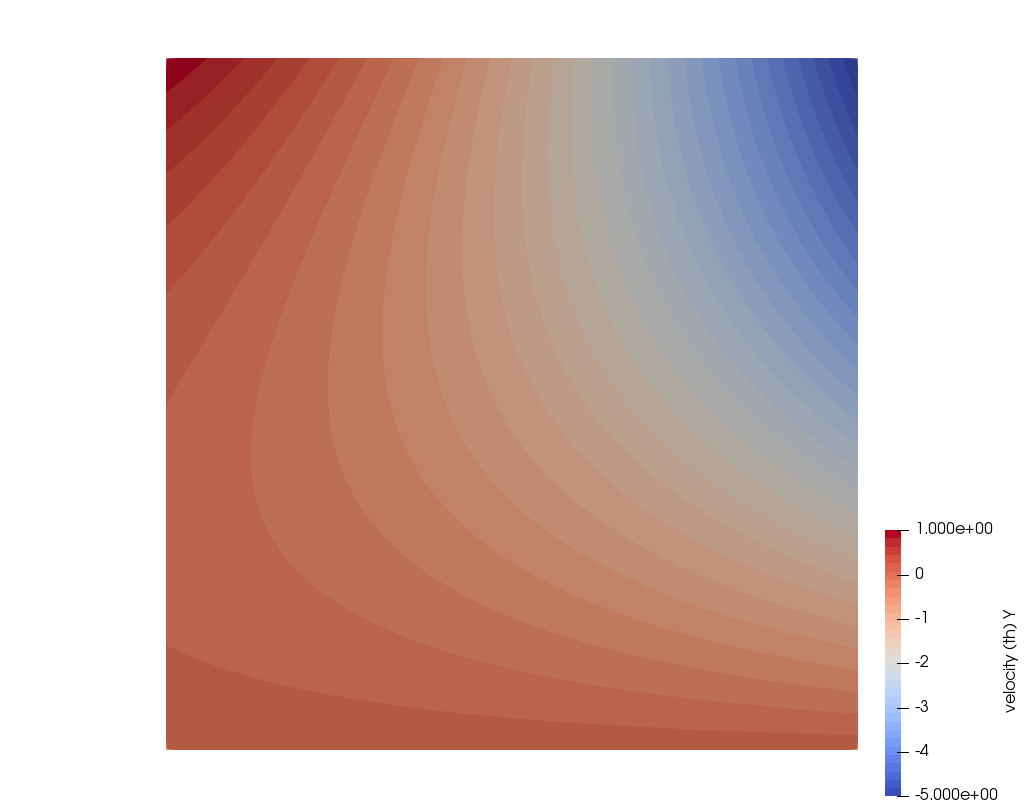
\includegraphics[width=5cm]{python_codes/fieldstone_22/results/vth}
%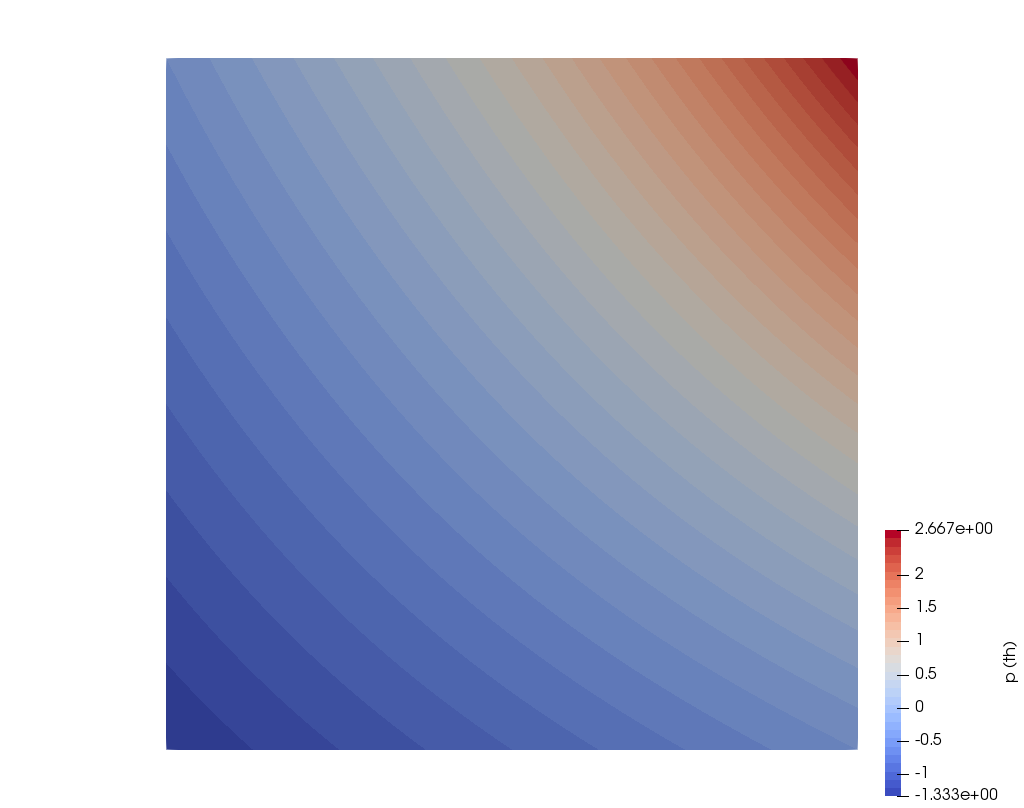
\includegraphics[width=5cm]{python_codes/fieldstone_22/results/pth}

%-----------------------------------------
\subsection*{The falling block experiment} 

The setup is desscribed in \cite{thba19}.

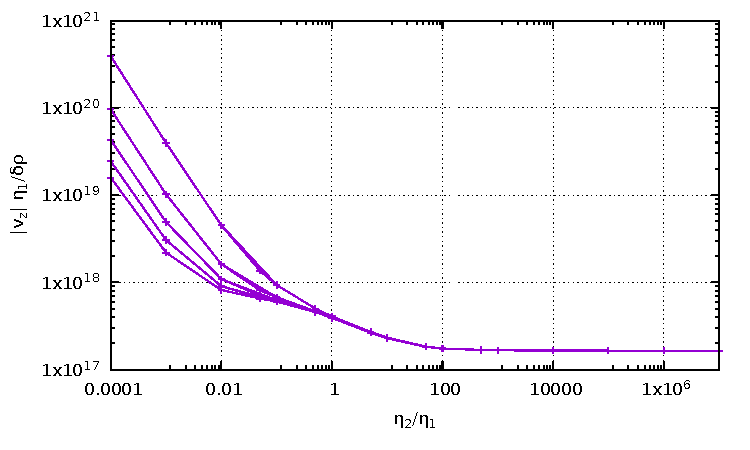
\includegraphics[width=10cm]{python_codes/fieldstone_22/results/case3/fallingblock.pdf}






